\section{Performance Evaluation}
\label{sec:performance}

\subsection{Evaluation protocol and metrics}
Each run is evaluated once on the 2{,}005-image test split, using the checkpoint chosen on validation
macro-F1. With $\mathrm{TP}_c$, $\mathrm{FP}_c$, $\mathrm{FN}_c$ counted one-vs-rest for each class $c$:
\begin{itemize}
  \item \textbf{Accuracy}: fraction of correct predictions. This is the official MedMNIST metric, but it is
        dominated by \texttt{nv}.
  \item \textbf{Balanced accuracy}: mean per-class recall,
        $\frac1K\sum_c \mathrm{TP}_c/(\mathrm{TP}_c+\mathrm{FN}_c)$.
  \item \textbf{Macro-F1} (primary): unweighted mean of per-class
        $F_1 = 2\,\mathrm{P}_c\mathrm{R}_c/(\mathrm{P}_c+\mathrm{R}_c)$. Every class counts equally, including
        melanoma and the rare classes.
  \item \textbf{Macro AUC}: mean one-vs-rest area under the ROC curve. It is threshold-free and is the second
        official MedMNIST metric.
  \item \textbf{Expected calibration error (ECE)}~\cite{guo2017}: with 15 equal-width confidence bins $B_m$,
        $\mathrm{ECE} = \sum_m \frac{|B_m|}{n}\,\big|\mathrm{acc}(B_m) - \mathrm{conf}(B_m)\big|$. Lower is better.
        This matters when predicted probabilities are used for triage.
  \item \textbf{95\% confidence intervals}: percentile bootstrap over 1{,}000 resamples of the test set.
\end{itemize}
\textbf{Test-time augmentation (TTA)} averages the softmax outputs over the 8 dihedral transforms of each
image (4 rotations $\times$ \{identity, horizontal flip\}). These are exactly the symmetries the model saw
during training. Whether the best model uses TTA is also decided on the validation split.


\subsection{Training dynamics}
Figure~\ref{fig:curves} (left) shows validation macro-F1 per epoch for all seven runs. Three regimes are
visible:
\begin{itemize}
  \item \textbf{Scratch.} The SimpleCNN learns slowly and noisily, climbing from 0.20 to its best value of 0.49 at
        epoch~\ScratchBestEpoch, then plateauing. Early stopping ended it at epoch 27.
  \item \textbf{Frozen backbones} plateau within about five epochs at 0.55 (ResNet-50) and 0.59 (EfficientNet-B0).
        A linear head on fixed ImageNet features has little capacity to adapt to dermatoscopic texture.
  \item \textbf{Fine-tuned backbones} pass 0.70 by epoch 3--4 and keep improving, with ResNet-50 reaching 0.795 at
        epoch \RFineBestEpoch.
\end{itemize}
Epoch-to-epoch swings of $\pm0.03$--$0.05$ are expected. The validation split has only 12 \texttt{df} and 14
\texttt{vasc} images, so a single image changes that class's recall by 7--8 points.

The loss curves of the selected model (Figure~\ref{fig:curves}, right) show no overfitting within 12 epochs: the
validation loss keeps falling until the selected epoch. The training loss stays \emph{above} the validation loss
because it is measured under augmentation, dropout, label smoothing and class weighting. The validation loss is
plain cross-entropy on clean images, so the two curves are not on the same scale.

\begin{figure}[H]
\centering
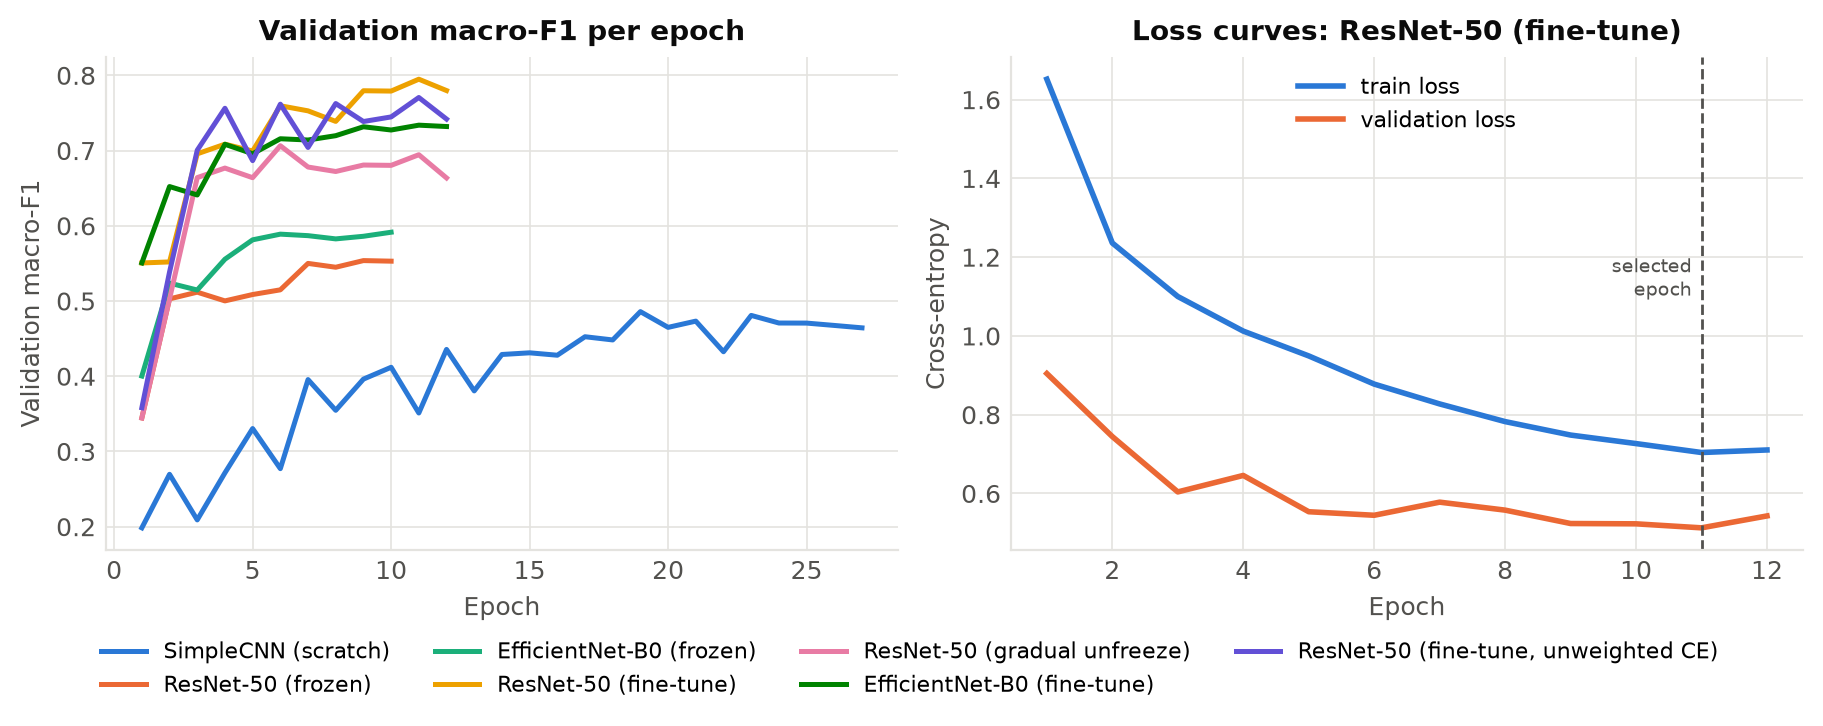
\includegraphics[width=\textwidth]{../results/figures/training_curves.png}
\caption{Left: validation macro-F1 per epoch for all runs. Right: training and validation loss of the selected
model (ResNet-50, full fine-tuning); the dashed line marks the checkpoint chosen on validation macro-F1.}
\label{fig:curves}
\end{figure}

\subsection{Main results}
Table~\ref{tab:results} and Figure~\ref{fig:comparison} summarise the test results (single view, i.e.\ without
TTA, so every run is compared on equal terms).

\begin{table}[H]
\centering
\caption{Test-set results of all runs (single view). Val F1 is the validation macro-F1 of the selected
checkpoint; macro-F1 is shown with its 95\% bootstrap CI. Bold: the model selected on validation.
Acc.\ = accuracy, Bal.\ = balanced accuracy, both in \%.}
\label{tab:results}
\footnotesize
\setlength{\tabcolsep}{3.5pt}
\resizebox{\textwidth}{!}{%
\begin{tabular}{lrrcrrrlrr}
\toprule
Run & Params & Trainable & Best ep. & Val F1 & Acc. & Bal. & Macro-F1 [95\% CI] & AUC & ECE \\
 & (M) & (M) & / run & (\%) & (\%) & (\%) & (\%) & & \\
\midrule
\inputrows{generated/results_table.tex}
\midrule
\multicolumn{5}{l}{Majority class (always \texttt{nv})} & \MajorityAcc & 14.3 & 11.5 & 0.500 & -- \\
\bottomrule
\end{tabular}}
\end{table}

\begin{figure}[H]
\centering
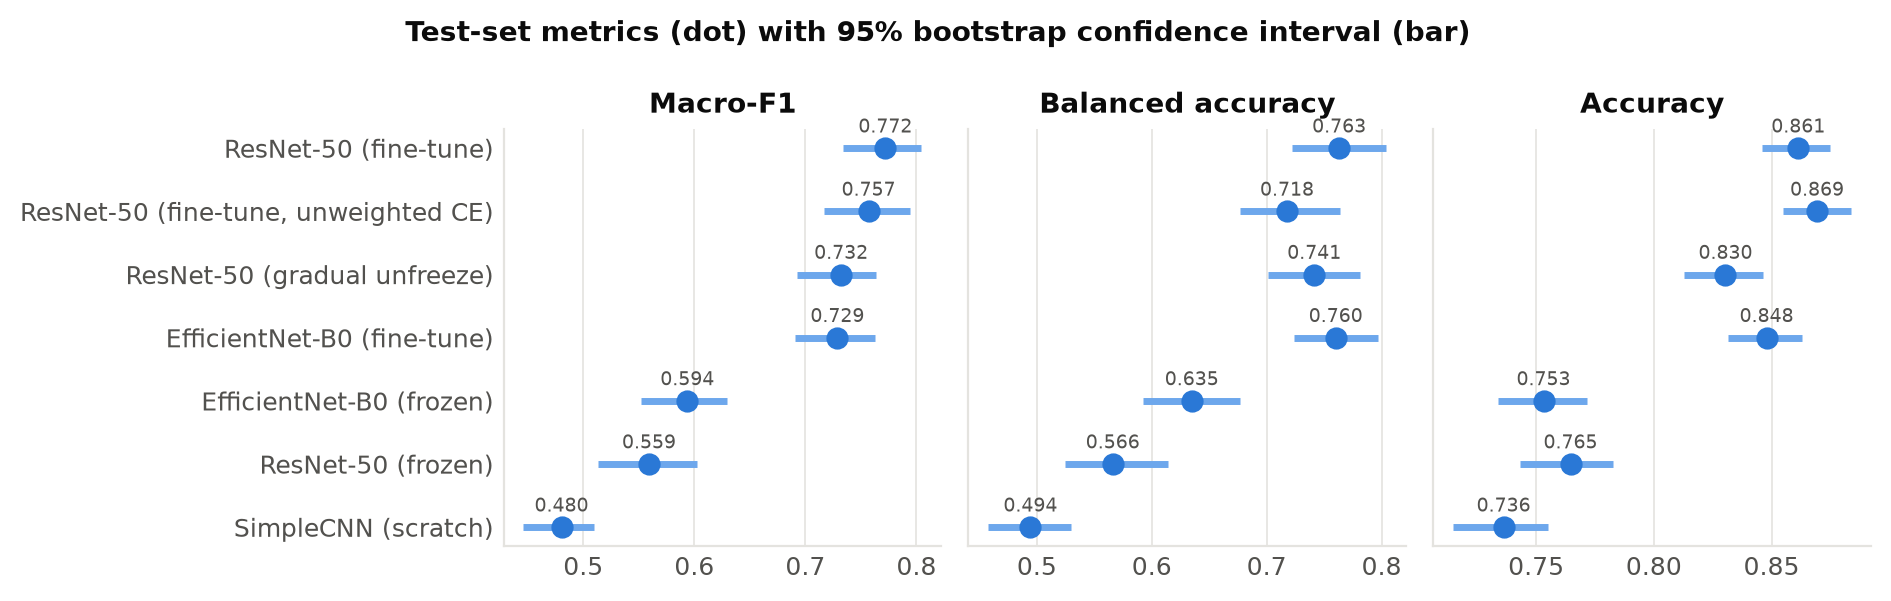
\includegraphics[width=\textwidth]{../results/figures/test_metric_comparison.png}
\caption{Test macro-F1, balanced accuracy and accuracy with 95\% bootstrap confidence intervals, sorted by
macro-F1.}
\label{fig:comparison}
\end{figure}

\paragraph{Finding 1: transfer learning is decisive.} The from-scratch SimpleCNN reaches \ScratchAcc\% accuracy,
only 6.7 points above the trivial majority classifier, and a macro-F1 of just \ScratchFOne\%. It never correctly
detects a single dermatofibroma (\texttt{df} F1 = \ScratchFOneDf). Fine-tuning an ImageNet ResNet-50 raises
macro-F1 to \RFineFOne\% (+29.2 points) and accuracy to \RFineAcc\%. The 95\% CIs, \RFineFOneCI{} against
\ScratchFOneCI{}, are far apart, so the gain is not a sampling artefact. With only 80--100 training images for the
rarest classes, features learned from 1.28\,M natural images~\cite{imagenet} give a far better starting point than
random initialisation.

\paragraph{Finding 2: frozen features are not enough; the domain shift has to be bridged.} Feature extraction
improves on scratch training (macro-F1 \RFrozenFOne\% for ResNet-50, \EFrozenFOne\% for EfficientNet-B0), but
full fine-tuning adds another \textbf{+21.3} (ResNet-50) and \textbf{+13.5} (EfficientNet-B0) points. This matches
the colour and texture shift found in Section~\ref{sec:data}. Dermatoscopic images look nothing like ImageNet
photographs, so the mid- and high-level filters must change, not just the classifier on top. The same pattern has
been reported for other medical-imaging transfer problems~\cite{raghu2019}.

\paragraph{Finding 3: ResNet-50 is the most accurate, EfficientNet-B0 the most efficient.} When frozen,
EfficientNet-B0 transfers better (\EFrozenFOne\% vs \RFrozenFOne\% macro-F1). After fine-tuning, ResNet-50 leads on
macro-F1 (\RFineFOne\% vs \EFineFOne\%) and accuracy (\RFineAcc\% vs \EFineAcc\%), while EfficientNet-B0 has a
slightly higher AUC (\EFineAUC{} vs \RFineAUC). EfficientNet-B0 does this with 5.9$\times$ fewer parameters,
10$\times$ fewer FLOPs and less than half the training time (\EFineTrainMin{} vs \RFineTrainMin\,min). It is the
better choice under a tight compute or deployment budget. The two macro-F1 CIs overlap (\EFineFOneCI{} vs
\RFineFOneCI), so the ResNet-50 lead is suggestive rather than conclusive.

\subsection{Effect of the transfer strategy: gradual unfreezing}
Gradual unfreezing reached \RGradFOne\% macro-F1, below full fine-tuning (\RFineFOne\%). Its best validation
epoch was epoch~\RGradBestEpoch, the end of the phase in which only \texttt{layer3}, \texttt{layer4} and the head
were trainable. Validation F1 did not improve after \texttt{layer2} and the stem were released. Two effects
explain this:
\begin{enumerate}
  \item the shared cosine schedule had already decayed the learning rate by then, so the lower stages, which
        start with $\le 2.5\times10^{-5}$, barely move;
  \item in a 12-epoch budget, half of the epochs are spent with most of the network frozen.
\end{enumerate}
The main purpose of gradual unfreezing is to protect pretrained features from large early gradients. In full
fine-tuning, warm-up and discriminative learning rates already provide that protection. Gradual unfreezing still
has advantages: it is about 30\% cheaper (\RGradTrainMin{} vs \RFineTrainMin\,min) and has the highest
single-view AUC among the class-weighted ResNet runs (\RGradAUC). With a longer budget, or with a separate
schedule restarted for each newly unfrozen stage, the gap would likely narrow.

\subsection{Ablation: class-weighted loss}
\label{sec:ablation}
Removing the class weights (E7 vs E4, everything else identical) shows a clear trade-off:

\begin{table}[H]
\centering
\caption{Class-weighted vs unweighted cross-entropy (ResNet-50, full fine-tuning, single view).}
\label{tab:ablation}
\small
\begin{tabular}{lrrrrrrr}
\toprule
Loss & Acc.\ (\%) & Bal.\ acc.\ (\%) & Macro-F1 (\%) & AUC & ECE & F1 \texttt{df} & F1 \texttt{vasc} \\
\midrule
weighted ($\sqrt{\text{inv.\ freq.}}$) & \RFineAcc & \textbf{\RFineBalAcc} & \textbf{\RFineFOne} & \RFineAUC & \RFineECE & \textbf{\RFineFOneDf} & \textbf{\RFineFOneVasc} \\
unweighted & \textbf{\RNoWAcc} & \RNoWBalAcc & \RNoWFOne & \textbf{\RNoWAUC} & \textbf{\RNoWECE} & \RNoWFOneDf & \RNoWFOneVasc \\
\bottomrule
\end{tabular}
\end{table}

Class weighting raises balanced accuracy by 4.5 points and macro-F1 by 1.5 points. The gain comes from the two
rarest classes (\texttt{df} +6.0 and \texttt{vasc} +5.3 F1 points). The cost is a little accuracy on the
majority classes (overall accuracy $-0.8$, \texttt{nv} F1 \RFineFOneNv{} vs \RNoWFOneNv) and much worse
calibration (ECE \RFineECE{} vs \RNoWECE). Weighting deliberately shifts probability mass towards rare classes,
so the raw softmax outputs no longer estimate true class frequencies. The unweighted model has the best AUC of
all runs (\RNoWAUC), so its \emph{ranking} of images is excellent. Its default arg-max decision rule simply
favours \texttt{nv}. In practice: if calibrated risk scores are needed, train unweighted and tune per-class
thresholds on validation; if balanced detection with a plain arg-max is needed, use weighting. The macro-F1
CIs overlap (\RFineFOneCI{} vs \RNoWFOneCI), so the macro-F1 difference is small relative to test-set noise.

\subsection{Test-time augmentation}
Averaging over the 8 dihedral views (Appendix, Table~\ref{tab:tta}) improves accuracy (+0.7 to +1.9 points) and
macro-AUC (+0.003 to +0.010) for \emph{every} run. It improves macro-F1 for six of the seven runs (+1.9 to +3.3
points; frozen EfficientNet-B0 is essentially unchanged at $-0.1$), at 8$\times$ the inference cost. For the selected model, TTA also
raised validation macro-F1 (0.795 $\rightarrow$ 0.810), so the final model uses TTA, a decision made on
validation only. Its final test performance is:

\begin{center}
\begin{tabular}{lll}
\toprule
\multicolumn{3}{c}{\textbf{Final model: ResNet-50, full fine-tuning, 8-view TTA (test set, n = 2{,}005)}} \\
\midrule
Accuracy & \textbf{\RFineAccTTA\%} & 95\% CI \RFineAccTTACI \\
Balanced accuracy & \textbf{\RFineBalAccTTA\%} & 95\% CI \RFineBalAccTTACI \\
Macro-F1 & \textbf{\RFineFOneTTA\%} & 95\% CI \RFineFOneTTACI \\
Macro AUC & \textbf{\RFineAUCTTA} & 95\% CI \RFineAUCTTACI \\
Cohen's $\kappa$ / ECE & \RFineKappaTTA{} / \RFineECETTA & \\
\bottomrule
\end{tabular}
\end{center}

\subsection{Per-class analysis of the final model}
\begin{table}[H]
\centering
\caption{Per-class test performance of the final model (ResNet-50 fine-tuned, 8-view TTA).}
\label{tab:perclass}
\begin{tabular}{lrrrrr}
\toprule
Class & Support & Precision (\%) & Recall (\%) & F1 (\%) & AUC \\
\midrule
\inputrows{generated/per_class_table.tex}
\bottomrule
\end{tabular}
\end{table}

\begin{figure}[H]
\centering
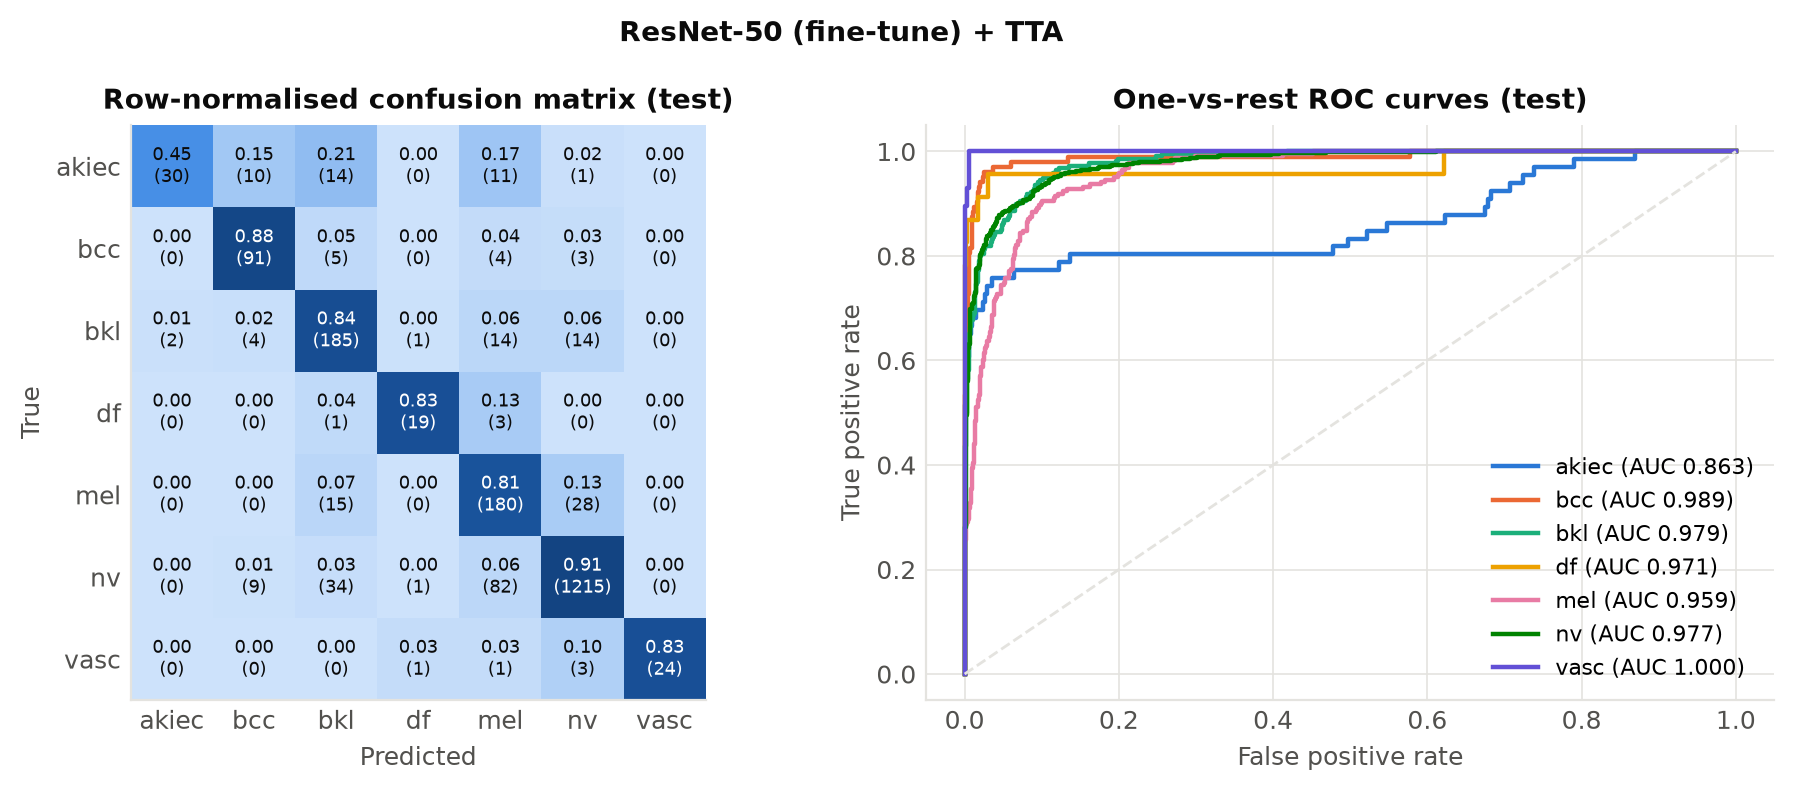
\includegraphics[width=\textwidth]{../results/figures/best_confusion_roc.png}
\caption{Final model on the test set: row-normalised confusion matrix (counts in brackets) and one-vs-rest ROC
curves.}
\label{fig:confusion}
\end{figure}

Table~\ref{tab:perclass} and Figure~\ref{fig:confusion} show where the model succeeds and fails.
\begin{itemize}
  \item \textbf{Strong classes.} \texttt{nv} (F1 \BestFOneNv\%), \texttt{vasc} (\BestFOneVasc\%, with 100\%
        precision), \texttt{df} (\BestFOneDf\%) and \texttt{bcc} (\BestFOneBcc\%). The visually distinctive
        \texttt{vasc} and \texttt{bcc} classes reach AUC \BestAUCVasc{} and \BestAUCBcc{}.
  \item \textbf{Melanoma} has recall \BestRecMel\% and precision \BestPrecMel\%. Of the 223 melanomas, 28 are
        called \texttt{nv} and 15 \texttt{bkl}. In the other direction, 82 nevi (6.1\% of all nevi) are flagged as
        melanoma, which accounts for most of its false positives. For a screening aid, this direction of error
        (over-calling melanoma rather than missing it) is the safer one.
  \item \textbf{Actinic keratoses (\texttt{akiec})} are the weakest class. When the model predicts \texttt{akiec}
        it is almost always right (precision \BestPrecAkiec\%), but it finds only \BestRecAkiec\% of them. Missed
        cases go to \texttt{bkl} (14), \texttt{mel} (11) and \texttt{bcc} (10). \texttt{akiec} and \texttt{bkl}
        are both scaly, keratinocytic lesions, and pigmented actinic keratoses can mimic melanoma. Its lower AUC
        (\BestAUCAkiec) shows that the class is hard to separate at any threshold, not only at the arg-max.
\end{itemize}

Figure~\ref{fig:heatmap} compares per-class F1 across all runs. Fine-tuning improves every class. The largest
gains are on \texttt{bcc} ($+0.29$ over frozen ResNet-50), \texttt{df} ($+0.36$) and \texttt{vasc} ($+0.30$),
the classes with the most distinctive local structure.

\begin{figure}[H]
\centering
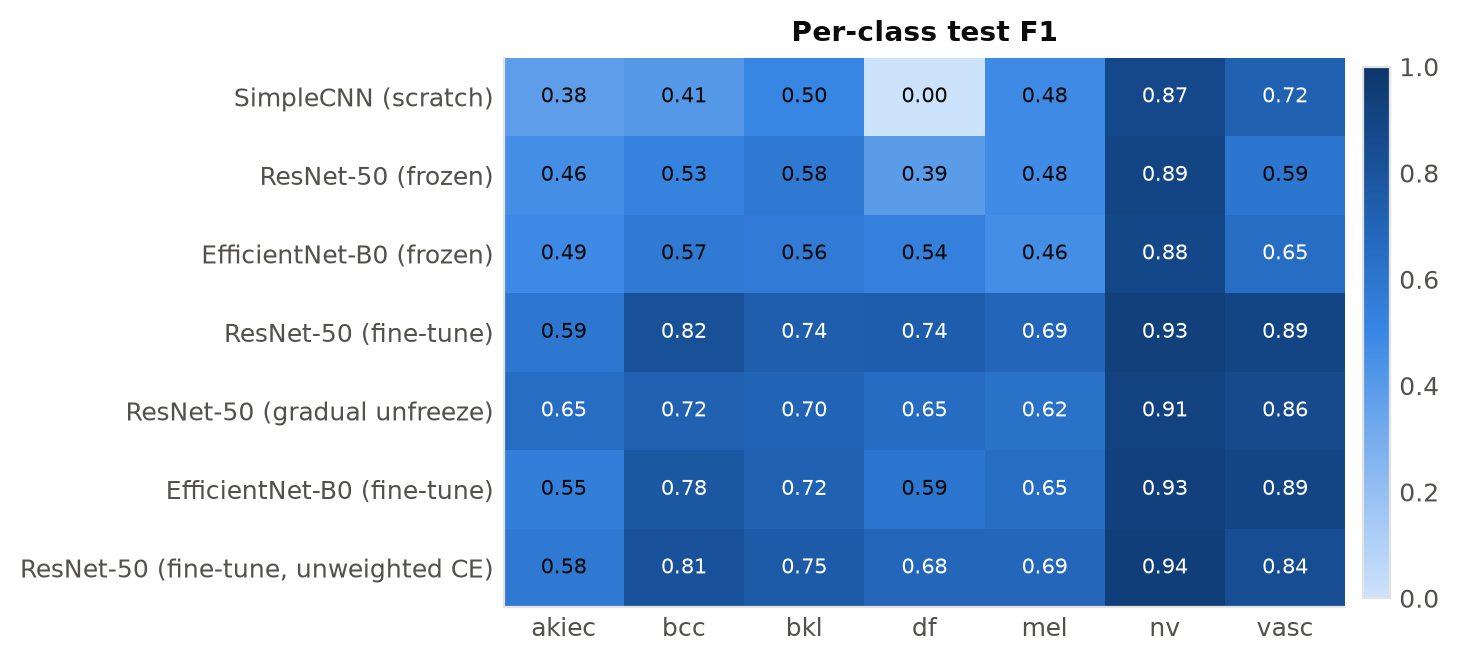
\includegraphics[width=0.85\textwidth]{../results/figures/per_class_f1_heatmap.png}
\caption{Per-class test F1 (single view) for every run.}
\label{fig:heatmap}
\end{figure}

\subsection{Calibration}
\begin{figure}[H]
\centering
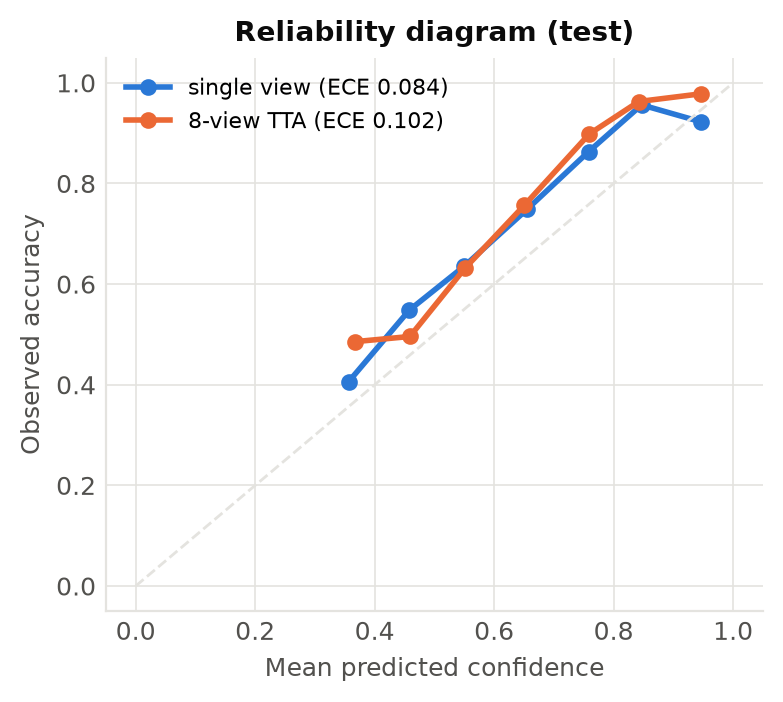
\includegraphics[width=0.42\textwidth]{../results/figures/best_reliability.png}
\caption{Reliability diagram of the final model (10 bins with at least 10 images). Points above the diagonal
indicate under-confidence.}
\label{fig:reliability}
\end{figure}
The reliability diagram (Figure~\ref{fig:reliability}) lies \emph{above} the diagonal: predictions made with
55--65\% confidence are correct 63--75\% of the time, so the model is \emph{under}-confident (ECE \RFineECE{} single
view, \RFineECETTA{} with TTA). The causes are label smoothing (which caps the target probability at 0.957),
class weighting (Section~\ref{sec:ablation}) and, for TTA, averaging over views, which further softens the
outputs. Ranking quality (AUC) is unaffected. If calibrated probabilities are needed, one temperature parameter
fitted on the validation split (temperature scaling~\cite{guo2017}) would correct this without changing any
prediction.

\subsection{Explainability: Grad-CAM and learned representations}
\begin{figure}[H]
\centering
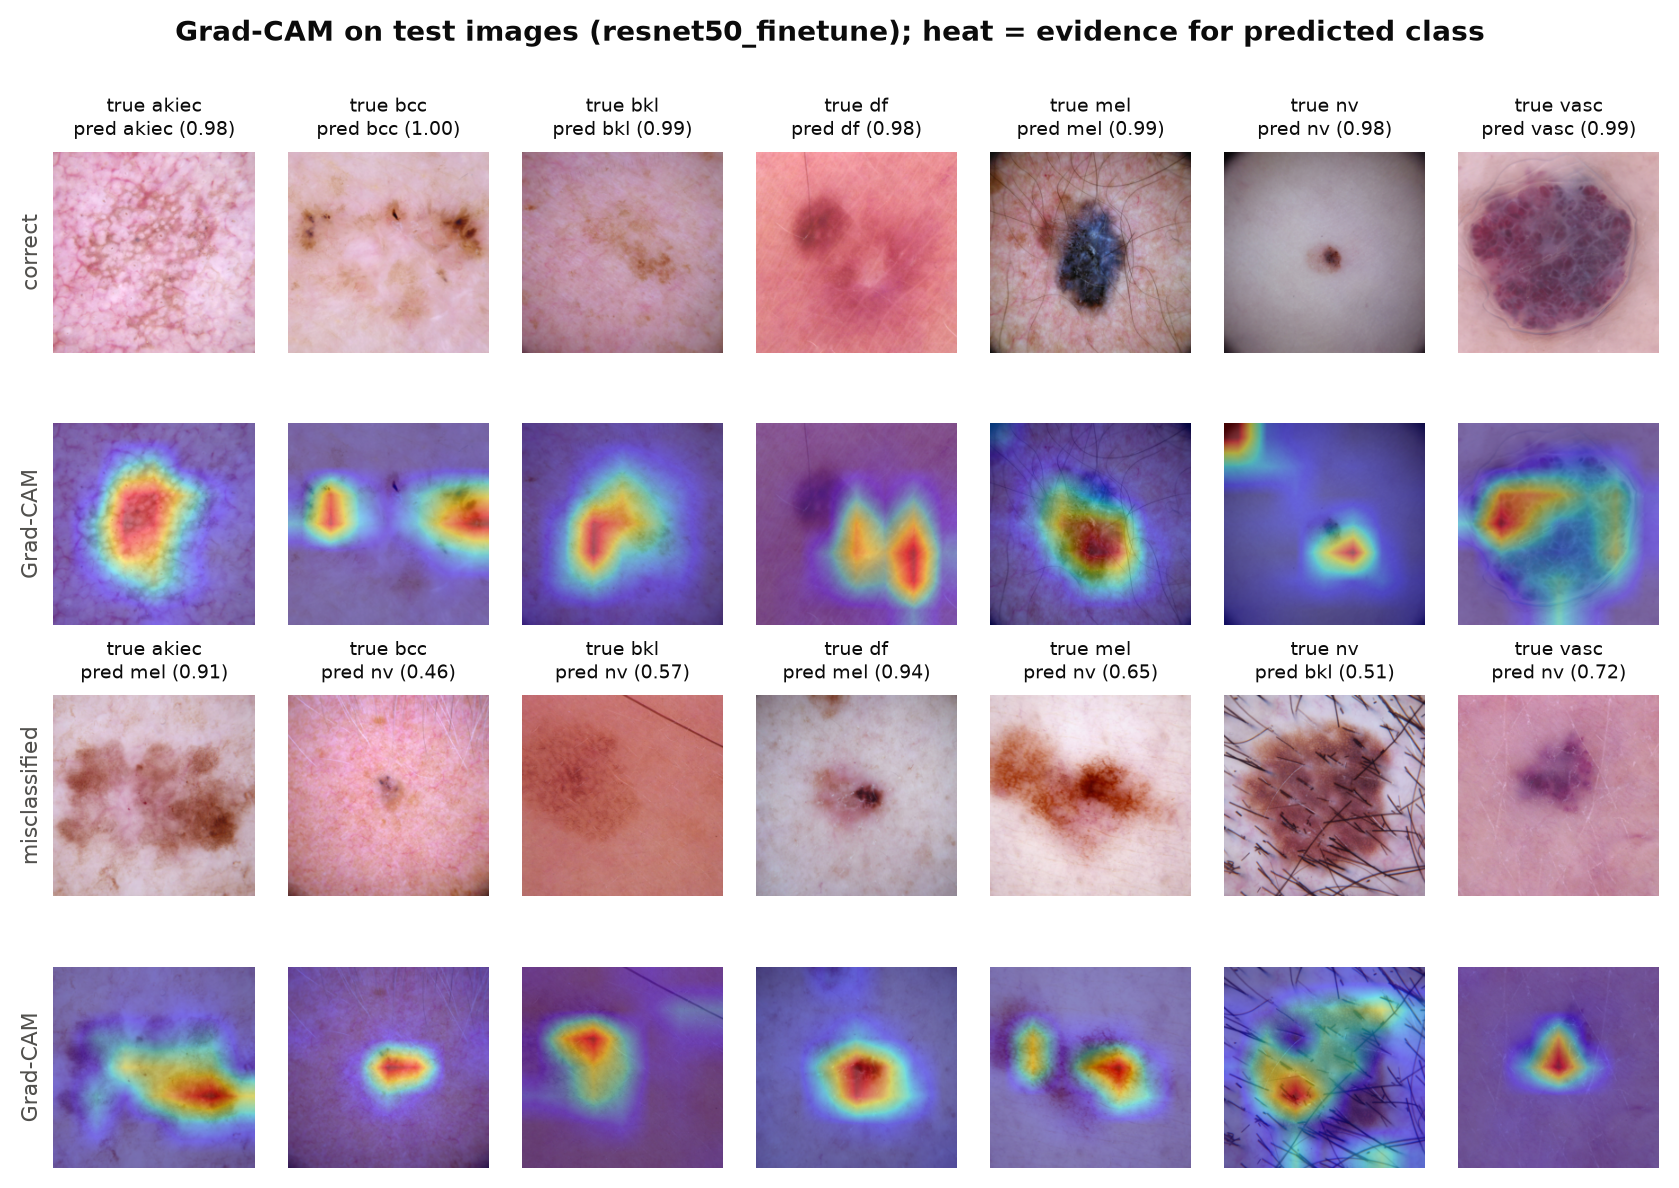
\includegraphics[width=\textwidth]{../results/figures/gradcam_resnet50_finetune.png}
\caption{Grad-CAM~\cite{gradcam} of the final ResNet-50 (last bottleneck block of \texttt{layer4}) on test images.
Rows 1--2: confidently correct examples per class; rows 3--4: one misclassified example per class
(single-view probabilities).}
\label{fig:gradcam}
\end{figure}

\textbf{Grad-CAM} (Figure~\ref{fig:gradcam}) shows that, for most correct predictions, the evidence lies on the
lesion itself:
\begin{itemize}
  \item the scattered pigmented foci of the basal cell carcinoma;
  \item the blue-black centre of the melanoma;
  \item the red-purple lobules of the vascular lesion;
  \item the central lesion area of the actinic keratosis.
\end{itemize}
Two observations call for caution. First, in the correctly classified nevus, a strong activation also sits in the
\emph{dark vignetted corner} of the image, which points to a possible acquisition-artefact shortcut. Second, for
the nevus misclassified as \texttt{bkl}, the heat is spread over the \emph{hairs} covering the lesion. Both point to
hair removal and vignetting-aware cropping as useful preprocessing. Five of the seven misclassified examples are
low-confidence, genuinely ambiguous cases (0.46--0.72). The two exceptions are a pigmented \texttt{akiec}
(0.91) and a \texttt{df} (0.94), both predicted as melanoma.

\begin{figure}[H]
\centering
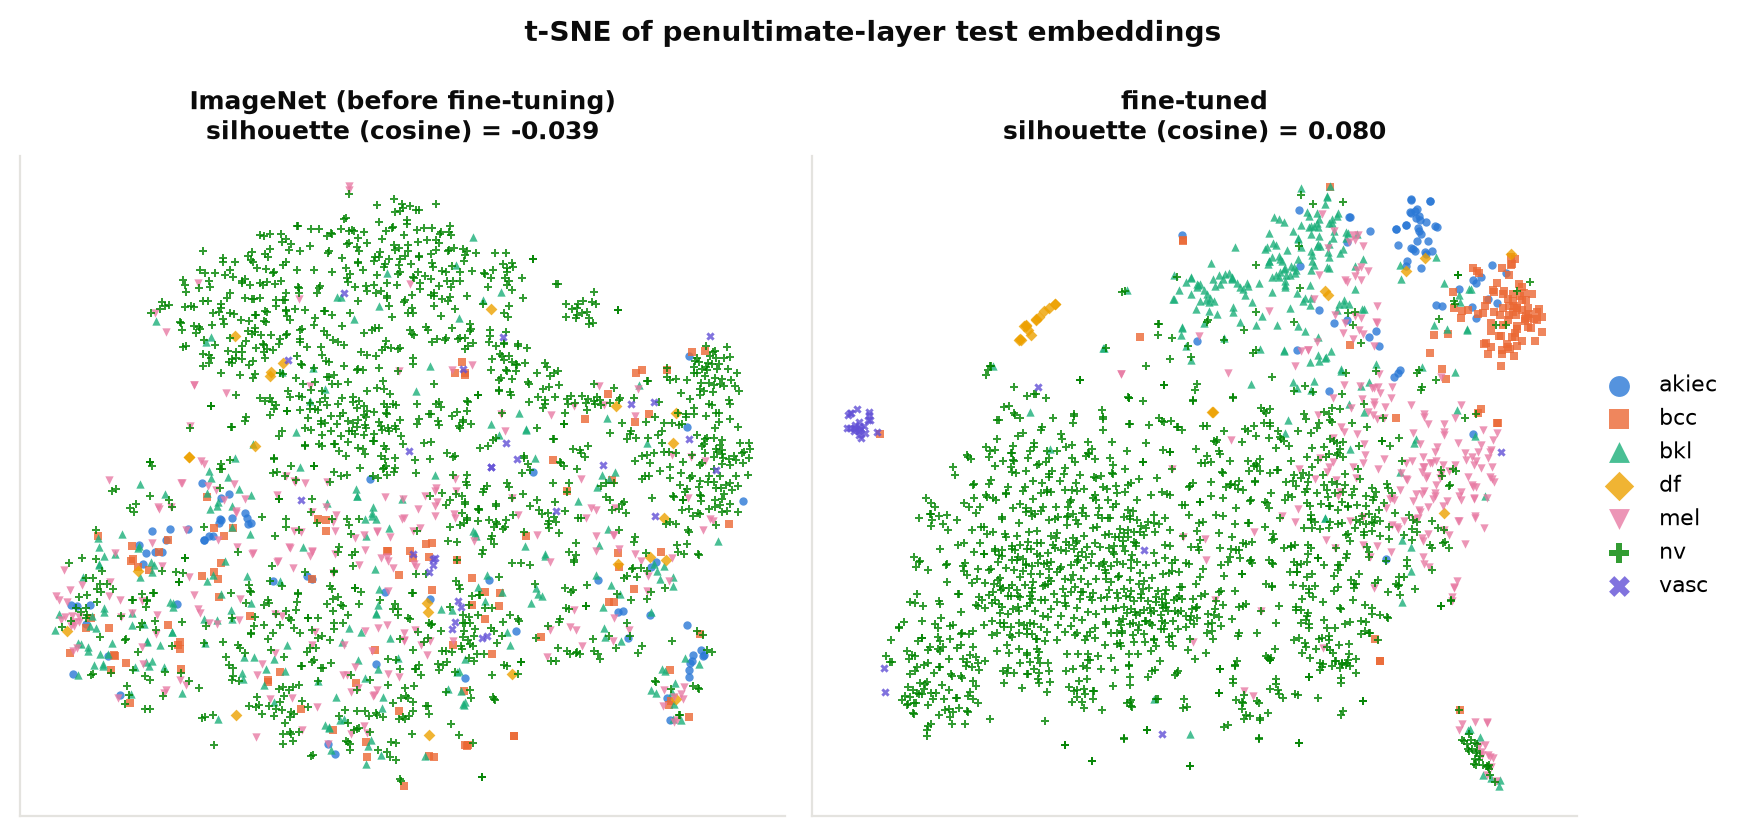
\includegraphics[width=\textwidth]{../results/figures/tsne_resnet50_finetune.png}
\caption{t-SNE~\cite{tsne} of 2048-D penultimate-layer embeddings of the 2{,}005 test images, before (ImageNet
weights) and after fine-tuning. Marker shape and colour both encode the class.}
\label{fig:tsne}
\end{figure}

\textbf{Embeddings.} Figure~\ref{fig:tsne} shows what fine-tuning changes inside the network. With ImageNet
weights, all classes are intermixed (cosine silhouette \SilImageNet). After fine-tuning, \texttt{vasc},
\texttt{df}, \texttt{bcc}, \texttt{akiec} and \texttt{bkl} form compact, separate clusters, and the silhouette
becomes positive (\SilFineTuned). Melanoma occupies a region that borders and overlaps the large nevus cloud,
which matches the \texttt{mel}$\leftrightarrow$\texttt{nv} confusions that dominate the error analysis.

\subsection{Comparison with published DermaMNIST results}
\begin{table}[H]
\centering
\caption{Comparison with the official MedMNIST v2 DermaMNIST benchmark~\cite{medmnistv2}. The MedMNIST v2
baselines were trained on the 28$\times$28 images (the ``224'' variants use 28$\times$28 images upsampled to
224$\times$224); our models use the native 224$\times$224 MedMNIST+ images.}
\label{tab:benchmark}
\small
\begin{tabular}{llrr}
\toprule
Source & Method & Test ACC & Test AUC \\
\midrule
MedMNIST v2 & ResNet-18 (28) / ResNet-18 (224) & 0.735 / 0.754 & 0.917 / 0.920 \\
MedMNIST v2 & ResNet-50 (28) / ResNet-50 (224) & 0.735 / 0.731 & 0.913 / 0.912 \\
MedMNIST v2 & auto-sklearn / AutoKeras & 0.719 / 0.749 & 0.902 / 0.915 \\
MedMNIST v2 & Google AutoML Vision & 0.768 & 0.914 \\
\midrule
This work & SimpleCNN, scratch (E1) & 0.736 & 0.908 \\
This work & EfficientNet-B0, fine-tuned (E5) & 0.848 & 0.959 \\
This work & ResNet-50, fine-tuned (E4) & 0.861 & 0.955 \\
This work & \textbf{ResNet-50, fine-tuned + TTA (final)} & \textbf{0.870} & \textbf{0.962} \\
\bottomrule
\end{tabular}
\end{table}

Our scratch baseline lands in the same range as the MedMNIST v2 baselines (0.72--0.77 ACC), which is a useful
sanity check of the pipeline. The fine-tuned models improve on the best published baseline by about
10 accuracy points and 0.04 AUC. This gain combines two factors, pretraining and native-resolution input, and
the comparison does not separate them. For the effect of pretraining alone, Table~\ref{tab:results} (identical
data and resolution) is the controlled comparison.

\subsection{Computational cost}
All seven runs together took \TotalTrainMin{} minutes of training on the GTX 1660 SUPER (Appendix,
Table~\ref{tab:compute}). A full ResNet-50 fine-tuning epoch takes \RFineEpochTime\,s and peaks at 3.9\,GB of GPU
memory. EfficientNet-B0 needs \EFineEpochTime\,s per epoch, and feature extraction only \EFrozenEpochTime--\RFrozenEpochTime\,s,
because no gradients flow through the backbone.
